%!TEX encoding = UTF-8 Unicode
\documentclass[11pt]{article}
% \setlength{\textwidth}{15cm}

% The name of the artefact produced
\def\theartefact{TravleTag}
% Default section name
\def\sectionautorefname{Section}


\author{Eivind Elseth}
\title{First draft of the project description of \theartefact}

%Font packages (input font, and font encoding
\usepackage[utf8]{inputenc}
\usepackage[T1]{fontenc}

\usepackage[pdftex]{graphicx}
\usepackage[english]{babel}



\usepackage{fancyhdr}
\usepackage{setspace}
\usepackage{graphics}


% Package for mathematical signs
\usepackage[geometry]{ifsym}

% Package for setting margin sizees
\usepackage{anysize}
\marginsize{3cm}{2cm}{1cm}{1cm}

% Siteringspakkene
\usepackage{hyperref}
\usepackage{natbib}
%\bibpunct{[}{]}{;}{a}{,}{,}


\setlength{\headheight}{15pt}
\usepackage{float}

\pagestyle{fancy}
\lfoot{\today} 
\cfoot{} 
\rfoot{\thepage}





\begin{document}
% \selectlanguage{norsk}

\doublespacing

\maketitle
\abstract{The first draft of the project description of my master thesis. The thesis will describe the design and implementation of \theartefact, and evaluate how it fulfills the goals set.}

\newpage
\tableofcontents

\newpage

\section{Introduction} \label{sec:Introduction}
If one wants to create an app to help people find interesting places and shops, good places to eat or drink coffee, and places where one can find lodging or exciting activities, 
one either needs to build a data set containing this information or find some source that provides this information.

For small developers it isn't feasible to build and maintain data source of that size. The task is simply to big. 
Inn addition to this comes the fact that if every developer was to create his own data source there would be a whole lot of redundant data sets, and a lot of redundant work, since there would be a lot of overlap between the information in the different sets.

There exists some data sources with this kind of information, Hotels.com\footnote{\url{http://www.hotels.com}} and VisitNorway and its subsites\footnote{\url{http://www.visitnorway.com}, \url{http://www.visitbergen.com/no/} etc. } are examples of sites that provide information about travel and tourism in Norway.
But the information on these types of sites is proprietary, meaning that the site owns the information and might not allow others to reuse it in other applications. If it is available it is usually limited to the type of information relevant to the sites own needs, and available through an API( Application Programming Interface).

Since it is not feasible for small developers and smaller projects to build a extensive data source, and since it it presently hard to find an open data set containing this type of information,  one must believe that there are a lot interesting ideas that are never realized.

To realize these projects we want to create a data source that is reusable, and open to developers. The data store will store information about points of interest(POI) using RDF(Resource Description Framework). 
The use of RDF will promote reusability since using information from one RDF store in another context only requires the user to align the ontologies used for the different graphs. 

Ontologies are also powerful in the way that they express the relationships between entities in the store. They store information in such a way that one can reason about the content of the store. 
This means that one can say such things as "People that have released music on CDs are artists.". If one later wants to find all the artist, it is possible to find people who have released CDs, event if it isn't said explicitly in the data store that they are artists or some subclass of artist.
The fact that ontologies users reason about the content of ontologies means that building ontologies is the domain of experts. Care needs to be taken to ensure than one maintains the truth in the knowledge base.

The main difficulty we are going to face in creating this data source is finding a way for users to save information about a POI in a way that is both simple enough that they can do it without extensive training, a powerful enough that they don't feel restricted in what they can say.
We need to have a way of generating light weight ontologies in such a way that they can be reasoned with, generalized, and reused. We also need an interface through which the users can interact to generate a knowledge base.


\section{Literature review} \label{sec:Literature} 
In this section we are going to go through some of the literature on how to create ontologies from non-semantic data.
This process of semantic lifting will be central to the thesis. 
The main part of this thesis will cover lifting semantic data from tags, but we will also cover semantic lifting from dynamic sources such as spreadsheets, which can allow the data store to have dynamic data which changes over time.

\subsection{Ontology and folksonomy}
One of the central concepts in semantic web technology is that of the ontology. 
In philosophy Ontology is the branch dealing with the study of which things 'exists', and if it is possible to categorize these things. 
For artificial intelligence \citet{Gruber1993} explained it as "an explicit specification of a conceptualization". 
That is than one commits to a given conceptualization of the domain in question, and formalize how we describe and reason about these conceptualizations. 
\citet{Pretorius2004} also gives a good overview of the history of the term, and show several of the interpretations and formalisms. 
One can also go to \citet{Noy1997} to find comparisons of several of the early ontologies, including WordNet which will be important in this thesis.

\citet{Shirky2007} criticizes the use of ontologies as a way of trying to enforce a structure on something that is by nature unstructured. 
He instead pushes the idea of common tagging. 
Part of the reason he criticizes the ontology approach is that it seem improbable that experts can know the needs of all the users a priori, and therefor that every ontology will prove to be inadequate.
%\citet{Doan2002} Tror ikke denne skal brukes
On the semantic web, ontologies are represented using collection of RDF( Resource Description Framework) triplets. 
These triplets are in the form of <subject, predicate, object>, much like simple declarative sentences \citep{Berners-Lee2001}. 
Each subject and predicate, and some objects, is represented by an URI( Universal Resource Identifier), which links to the resource that describes it.

While ontologies are formally constructed taxonomies, folksonomies are informal taxonomies generated by collecting tags or annotations from collaborative tagging systems on a given platform\citep{Tang2009}. 
\citet{Mika2005} has given a more formal definition of folksonomy where he sees a folksonomy as a set of tags T, 
$T \subseteq A \times C \times I$, where A is the set of users tagging, C is the set of tags, and I is the set of objects being tagged.
\citet{Gruber2007} suggested that one should add the source of the tag, and some kind of rating system to help filter out junk tags. 
\citet{Scerri2008} on the other hand suggests removing the objects being tagged from the ontology, 
seeing that the objects that are being described are not part of the tool to describe them.
Instead they like Gruber want to add the source of the tag, the number or times a tag occur, and the tagging behavior of each user.
\citet{Bang2008} explains the difference between ontologies and folksonomies by classifying them as a priori and a posteriori annotations. 
That is, ontologies are created by experts as ways on conceptualizing a domain, folksonomies on the other hand are samples of how people speak or think about a domain.
Folksonomies grew as a subject of research as it became popular for users to tag content on the internet with keywords they felt were relevant.

For users tags are convenient, since Adding additional tags can make it easier for humans to search and browse collections. This is especially true for multimedia content, which we don't yet have good tools for searching in \citep{Weinberger2008}.
Tags provide meta data about content in a way that makes sense to humans. From an information retrieval perspective this is interesting since it means that humans in some way add meaning to the content.
There however are several problems with using tags as the basis of a semantic web. \citet{Tang2009} mention several. 
Tags are supposed to be written in natural language, and natural language has words that are synonymes(words that are written in different ways, 
but mean the same), homonymes(words with different meanings that are written in the same way), or polynyms( a word that can have several meanings) 
making it unsuitable for computer reasoning since they are ambiguous \citep{Passant2008}. 
As \citet{Golder2005} mentions, users also operate on different levels of abstraction, which can make it harder to find interesting resources.
In addition to this comes the problem of non dictionary words, both new, or compound words, or simply words that have been misspelled\citep{Tonkin2006}.


There has been done a lot of research into how one can lift semantic data out of these unstructured tags.
\citet{Golder2005} has done research into the statistical analysis of tags. 
The analysis done here show that there seems to develop vocabularies of frequently used tags. 
This might help diminish the effect of misspelled and nonsense words. Similar findings were also reported by \citep{Shirky2007}

There has also been done research into automatic clustering. 
\citet{Mika2005} created clusters by creating weighted graphs, and compared using tag concurrence and actor interest as weights.  
\citet{Brooks2006} has done work an categorizing blogs entries by tags, to see if concurrence of tags indicated similar content. 
Using the most common tags did give some results, but only broad categories. The results were not better than extracting words that were given asserted to be relevant for the category.

\citep{Tang2009} tries to go further that clustering tags, and tries to build an hierarchical model from a folksonomy. 
They use a probabilistic model that takes into account the frequency and concurrence of tags and tries to generalize it to an ontology. 
The method does get good results in creating the hierarchy, but does also show som inappropriate sub/super category inferences.

\citet{Weinberger2008} suggests a method for removing ambiguity from tags,
 by suggesting additional tags to the user when the tag entered can belong to one of several distinct sets 

While there are many difficulties attached to merging the social and semantic web, and with lifting semantic data from tags, there are many researchers who stress the need for this \citep{Passant2007,Mika2005, Gruber2007}.

\subsection{WordNet and lexitags}
Lexitags \citep{Veres2011} utilizes a different approach for getting semantic meaning out of tags that the approaches mentioned until now. 
Instead of analyzing existing folksonomies and try to lift semantic data out of these tags, the idea presented is to turn it around and make users attach meaning to the tags at input time.
This is done by letting users disambiguate the tags by using WordNet synsets, an idea that was also mentioned by.

WordNet is a lexical reference system that stores words in sets of synonymes called synsets. The idea is to separate the word form from the word sense. 
The underlying assumption is that the user already knows English, is familiar with the concepts that are conveyed, 
and doesn't need definitions to understand, but can use synonymes to identify the meaning they want to convey\citep{Miller1990}.

In addition to storing these synsets WordNet also contains information about the semantic relationship between different concepts. 
The synonymy relationship is obviously contained within each synset, 
though it should be mentioned that the definition used in WordNet is not one where substitution never changes the truth value of a sentence. 
WordNet uses a weaker definition where two word forms can be seen as synonymes in relation to some semantic context. 
The antonymy relationship is another relationship between word forms. While the exact definition of antonymy is hard to pin down, the intuitive notion that an antonym to x is not-x will take us a long way\citep{Miller1990}.

WordNet also stores information about hyponymy and hypernymy, which is a relationship between concepts.
 A hypernym can be explained as a generalization of some concept, a hyponym on the other hand can be seen as a specialization of a concept. 
 \{tree\} can for example be seen as a hyponym of \{plant\}, and the reverse relation is a hypernymy relation \citep{Veres2010}.

The fact that WordNet separates sense and form is good for our purposes, as we are interested in the sense, not the form of the word. 
Mapping tags to synsets removes the ambiguity that arrises from multiple spellings. 
At the same time, since the mapping preserves the form of the tag this can still be kept for analysis if one finds that there are significant differences in how different forms of a synset is used\citep{Veres2011}.
By enforcing this mapping to WordNet lexitags also gets access to the hierarchical knowledge therein, and can create lightweight ontologies by using hypernyms of the tags as SuperTags, a method introduced by \citet{Veres2010}.
The mapping to WordNet also add some perks. There is a mapping between WordNet and Schema.org\footnote{\url{https://github.com/mhausenblas/schema-org-rdf}}, and between WordNet and the SUMO( Suggested Upper Merged Ontology)\citep{Niles2003}.

Using WordNet to ground the semantics of the tags was idea also suggested by \cite{Cattuto2008}. But \citet{Cattuto2008} suggested using a post hoc analysis of the tags in a social network, instead of enforcing the mapping though an interface.

One critique of WordNet comes from \citet{Mika2005} who points out that while WordNet can catch lexical sameness, it lacks cultural awareness. The example used was that of the tie between Noah and the ark.
This tie would be obvious for most humans, and would most lightly be caught through clustering tags, but would not be caught by WordNet.

\citet{Passant2008} has also suggested a system where taggs are disambiguated by the user at input time. A difference between the systems is that Passant and Laublet suggested using URIs to online resources for disambiguation.

\subsection{Dynamic datasources}
The ability to add semantic data through tags is important for the success of this project. 
But tags are a static source of information. 
The folksonomy it self is dynamic, in that new tags can be added or old tags can be removed, but the tags them self are not the subject of change.
We also want to look at the possibility to add datasources that can change over time.

One way to do this is through the use of database wrappers such as D2RQ, SquirrelRDF, and OpenLink Virtuose which are described by \citet{Hebeler2009Chp9}. 
\citet{Langegger2009a} also describes how one can gain similar access to spreadsheets through the use of the tool XLWrap-Server which they've developed.
As \citet{Langegger2009a} points out, it is important for the success of the semantic web that one strives to gain access to legacy data.
Many companies have information about such things as opening hours, menues, and prices stored in either relational data bases, or as spreadsheets.
If one can gain access to these, by getting the URIs where they can be found, one can use these tools to generate mappings and endpoints
which can be used to query the information within. 
Since these are the same sources as the companies use, one can expect the data to be updated continuously and to get access to up to date information.
The mappings however need to be created separately for each data source, so we need to look at if this can be done easily enough for novice users.

\section{Research problem} \label{sec:Research}
In this project we want to try to create an artefact that will allow users to add content to a knowledge base in such a way that this knowledge base in turn could be used to create a light weight ontology.

Creating an ontology, and mapping date to an ontology is in most cases the type of thing one uses experts for.

The plan is to create a web site on which users can describe the POI they want to describe using tags.
We will use lexitags to disambiguate the tags by mapping them to WordNet synsets or to concepts from DBpedia. 
One can also imagine doing some basic parsing of the user input to see if it can have some other known meaning, like being a phone number, geo coordinate, or an organisation number.

This way, we hope it will be possible to both maintain the exact thing the user said, and to create light weight ontologies from these tags. 
These ontologies are made possible from the WordNet and SUMO mappings. (!!!! INSERT SOME REFERENCES HERE !!!)

In this thesis we're going to attempt a different route. 
The goal is to see if we can create an interface that will allow users without knowledge about semantic technologies to create semantic data about different points of interest in such a way that it can be shared freely with others.


For my thesis I am going to develop a tool that will help gather information about businesses that might be of interest to tourists.
The thesis will mainly focus on technologies relating to semantic web, and on lifting semantic data from non semantic sources.
I will explore how much semantic data one can glean from user input, from users who don't have any in depth knowledge about the related technologies.

To achieve this a tool that allows users to input information in natural language using the lexitags interface will be created, and the tags used to see if these tags can be used to extract extra data automatically through existing web services.

(REWRITE) To answer this question I want to see if I can create a tool that, by utilizing the lexitags system, empower developers and business owners to produce semantic content. 

A  usability study will be performed to see if the tool can be successfully used by users without knowledge about semantic technologies. 
I hope to show that it is possible to get naive users to create and deploy semantic content.
This could be important as it would show that that proper tools could make creating semantic content available to non experts. This in turn would be important with regards to the proliferation of semantic encoding on the internet.




\section{Methodology} \label{sec:Methodology}
The thesis will utilize a design research methodology to perform its research. 
The guidelines provided in \citet{Hevner2004} will be followed to ensure that the process is rigorous.
The guidelines provided in this article are:
\begin{enumerate}
    \item \label{gl1}Design as an Artifact
    \item \label{gl2}Problem Relevance
    \item \label{gl3}Design Evaluation
    \item \label{gl4}Research Contributions
    \item \label{gl5}Research Rigor
    \item \label{gl6}Design as a Search Process
    \item \label{gl7}Communication of Research
\end{enumerate}

We will now explain how we intend to follow these guidelines in our project.
The first guideline says that a design research project should produce some artefact. For this project the artefact is \theartefact. 

The second guideline is justified in section \ref{sec:Research}, and has to do with the objective of a design research project. 
The goal as stated here should be to develop an artefact that is relevant for solving some business problem.

Design evaluation is also mentioned and this guideline stresses the need for rigorous evaluation of the artefact that has been developed.
There are several metrics that are possible for \theartefact, but we will focus on ease of use, and quality of the data.

The research contribution of this project will be \theartefact, which will contribute to solve the problem of how to get users to create semantic content, and how to create open user created knowledge bases for POI data.

The need for research rigor, which is mentioned in guideline \ref{gl5} will be followed by following the multimethodological approach suggested in \citet{Chen1990} and \citet{NunamakerJr1990}. 
This will be the topic of the following section.

Guideline \ref{gl6} says that design research should be a search process. 
In this context that means that one should explore the possible implementations of the artefact by iterating through phases of generating prototypes and testing these prototypes against the requirements of the project( as seen in figure \ref{GenerateTestCycle}, page \pageref{GenerateTestCycle}).
To attain this type of cycle we will chose a system development methodology which utilizes multiple iterations of building and testing.
The last guideline proposed has to do with clear communication of the results of the research. 
It is further proposed that one should take care to have several channels of communication with different levels of technical detail.
The reasoning is that we need to convince both the technical and the managerial communities. 

To conform to the seventh guideline one should communicate the results of ones research in such a way that it is accessible for the intended target audience.
For this thesis, the written thesis itself will be the technical document, documenting the process of designing and implementing the artefact, focusing on an academic audience.
The document talking to management will take the form of a presentation highlighting the benefits of a user generated knowledge base, and the potential business uses.

\begin{figure}[h]
    \begin{center}
        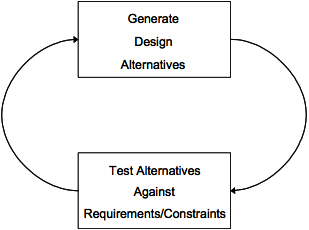
\includegraphics[width=0.60\textwidth]{Images/GenerateTestCycle.png}
        \caption{The generate/test cycle, from \protect \citet{Hevner2004}}
        \label{GenerateTestCycle}
    \end{center}
\end{figure}

For the design process we look to \citet{Chen1990}, who proposes four activities that interact in the development of information systems( See figure \ref{multi} on page \pageref{multi}). 
The paper suggests using a multimethodological approach where one moves between different research activities: Theory building, experimentation, observation and systems development.
By using these different approaches we can hope that we will catch important facets that might otherwise have been missed or over looked.   

\begin{figure}[h]
    \begin{center}
        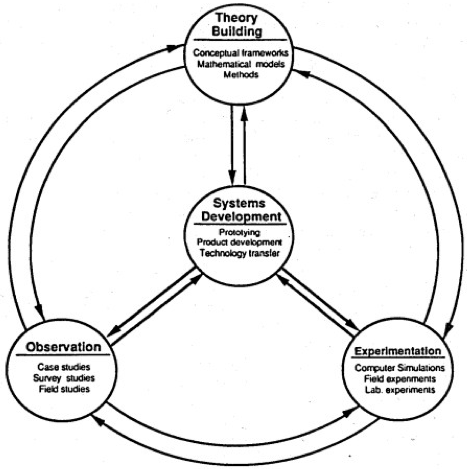
\includegraphics[width=0.60\textwidth]{Images/MultiMethodological.png}
        \caption{A multimethodological approach to IS research, from \protect \citet{Chen1990}}
        \label{multi}
    \end{center}
\end{figure}

% \citet{NunamakerJr1990} The article without the model
\subsection{Experimentation}
There are going to be three main experimentation phases in the thesis.
Before the main part of development starts we will look at how users want use tags to describe POIs.
During development we will periodically perform small usability tests to ensure that development is going the right way.
At the end of development we will also perform a larger user test, both to get data on the final product, and to more accurately judge how good the data created is.

To find out how we are going to design the artefact, we should get some data about how people tag.
To get this data we will perform an experiment on an early prototype of the system, with just the ability to add tags to describe a POI. 
The prototype could be a simple web interface with an input field, or could be as simple a notepad and a pen.
The choice of using a web interface or pen and paper would have to do with a cost benefit analysis, 
with the cost of creating the web prototype against the added validity of having an interface which is closer to the one the finished artifact will have.
Either way, this prototype will be used to perform experiments on the potential user groups. 

The experiment would consist of having a set of POIs that the subjects would be prompted to add information about. 
The subjects should be prompted beforehand to consider that they were adding tags that should help travelers find places they are interested inn, so they know the context of the tags.
These results can be analysed to see if there is a trend in the type of tags that were used. 
The results might help us find out what kind of framing we need for the artefact to get users to add the type of information we are interested in.

The usability studies performed during development will be performed periodically on small groups.
To keep these tests manageable we are going to use small test groups (3-4 users).
Using small test groups like this has been suggested by \citet{Nilsen2000}, and is somewhat backed by \citet{Bevan2003}. 
The claim made is that small user groups are enough to uncover problems with the artefact and that large groups are not needed
since the objective is to uncover pit falls, not to prove theories empirically.

At the end of development there will be a larger usability test to see if the artefact is simple enough in use that
users can express the things they want, and powerful enough to create RDF data of such a high quality that it can be reasoned about.


\subsection{Observation}
We are also going to carry out some observation of how people use tags to describe POIs on the web, and what type of information people want when they are planning to travel to a new location.
We will use two different methods to get this information.

We will look at how people actually use tags to talk about and describe POIs on the internet now by looking at web sites that allows users to add tags. 
Flickr\footnote{\url{http://www.flickr.com/}}, and Delicious\footnote{\url{http://delicious.com/}} are obvious places to start, 
but more research could be done to find better or additional sources before the observation begins.
Seeing that the internet is a virtual, not a physical, space, this type of observation is a close approximation of a field study, one of the methods suggested by \citet{Chen1990}.
The idea of analyzing data for finding interesting data for an ontology from Flicker tags was also explored by \citet{Schmitz2006}. 
In that article the attempt was to build an ontology by analyzing the co-occurrence of tags on Flickr as a whole. 
We will instead look at what type of tags people use, and their frequency of use.
This route has the advantage of being routed in the current use of tags. 

There would also be a large data set available, making it possible to potentially make strong statements about how tags are used to describe content.
Creating data sets for a set number of POIs can also be done simply through the sites APIs.
The disadvantage of this approach is that this would be a measure of how people use tags now. 
Depending on how one conceptualize, frame and present the artifact it is possible that the users would use tags differently in our system.

If we find that the current use if close to the one that we want to use in our artefact, 
or if we find that the type of tag used if platform dependent, 
then this will be an indication that setting a context for tagging might be enough.
If not then we might have to look into how we can convince users to tag differently when using our artefact.


Another source of information will be attained using surveys, one of the observational methodologies mentioned by \citet{Chen1990}.
This approach would consist of a survey sent to users with questions about what type of information they would want about different POIs if they were planning to visit an area.
The survey should contain open questions as to get the whole width of possible information that is wanted.
%% Experimentation was moved, read through and revise to remove inconsistencies 
Both this and the experiment should use different classes of POIs like stores, landmarks, restaurants, and hotels to capture a broad selection of tag usage. 
We should also look into the possibility of using the same POIs in the tag analysis from the web. 
This might not be applicable for the commercial POIs, which might not be as interesting for current taggers. 
But if we are able to find them, these would make it easier to compare results from between the different data sources.

Using the data from these three sources should give us ample information about how tags are used currently used to describe POIs, 
how subjects tag POIs when they are aware that they are tagging in the context of helping travelers, 
and what information people want when they think about traveling. 

The data gathered here will also be used to create the final success criteria for the artefact. 
The artefact will be successful if it can provide the types of data that users would want. 
The activities in this part should be seen in light of \citet{Chen1990} as research activities. 
Both the survey and looking at tag usage on the web are instances of observational studies.




\subsection{System development}
To ensure that the system development process is done in a reliable way we should find some structured process to try to follow.
For this project we are going to use a methodology called personal scrum, which is described by \citet{Pruitt2011}.
Personal scrum is a variation of SCRUM as introduced by \citet{Schwaber1995}. 
The main difference that SCRUM focuses on groups and group activities, while personal scrum is a variant with guidelines for how to do a SCRUM like methodology with a one person team.

The reason for choosing this methodology is that SCRUM is a time proven and popular methodology, with a strong emphasis on time boxing and incremental design.
To help the incremental design the requirements for the projects are translated into user stories,
short stories that says something about what users of the system should experience when using the system.
The methodology divides the development process into smaller chunks called sprints. 
A sprint consists of a set of user stories that the team commits to completed before the end of the sprint.
The set of user stories chosen for a sprint are the ones that are deemed the most critical, and which are not dependent on later stories. 
Each sprint finish with a new iteration of a complete product, which can be tested by a user group.
The fact that the methodology uses small sprints which ends with testable products make it a suitable choice.
We could for example switch between system development and experimentation or user testing, two of the activities in figure \ref{multi}.
We could also try out different representations of tags suggested in the literature \citep{Mika2005,Gruber2007,Scerri2008}, 
switching between developing the artefact and commenting on and expanding the literature.

\subsubsection{Initial spike}
Before development of the artefact can start we need to learn the tools we will be using. 
The main part of this phase will be exploring the API exposed by lexitags, and to get to know how to use the different methods.
Since a large part of the system will rely on interaction with lexitags, it is important to know the workings of the tool before designing the artefact.

\subsection{Theory building}
The theory building in the development of \theartefact\ will mainly consist of the evaluation of the artefact at the end.
After the final iteration we will be able to test the artefact against the requirements found in our surveys, 
and see if we are able to generate the type of information we want, and if the information is of a high enough quality.
At this point we will draw in data from all the activities to form a coherent theory.

Before this we might have to look at the theory for representing tags.
By examining and testing the models through development we can se if any of the current models are suitable for our artefact.
If this examination finds that none of the models are suitable for this kind of artefact, we might have to stop development
until such a model can be conceptualized.









\newpage
\bibliographystyle{apalike}	% Stilen jeg ofte bruker
\bibliography{library}		% Stien til .bib filen som inneholder referansene dine. Bare si ifra viss du trenger et eksempel.

\end{document}
